\section{Graphs}
{\tiny collection of vertices(nodes) connected pairwise by edges(arcs) \\
edges can be directed (also called arcs, 2-tuples or ordered pairs) and undirected (unordered pairs, or pair sets)
}\\
\scriptsize{applications}\\ 
{\tiny city maps, chemical formulas, neural networks, ANNs, electronic circuits, computer networks, infectious diseases, probability distributions, word semantics\\
food web, course dependencies, social media, scheduling, games, academic networks, inheritance relations in OOP, flow charts, financial transactions, world's languages, PageRank algorithm
}\\
\scriptsize{types}\\ {\tiny directed graph: with only directed edges, e.g. course dependencies\\
undirected graph: with only undirected edges, e.g. transportation(e.g. railway) networks\\
mixed graph: contains both directed and undirected edges (e.g. city map)\\
simple: there is only a single edge between 2 nodes\\
weighted: the edges have associated weights\\
complete: contains edges from each node to every other node\\
bipartite: has 2 disjoint sets of nodes, where edges are always across the sets\\
multi-graph: there are multiple edges (with the same direction) between a pair of nodes\\
hyper-graph: a single edge can link more than 2 nodes
}\\
\scriptsize{more definitions}\\ {\tiny endpoints: two nodes joined by that edge\\
incident: an edge is incident to a node if the node is one of its endpoints\\
adjacent/neighbors: two nodes are incident to the same edge\\
degree/valency: number of its incident edges\\
indegree: num of incoming edges\\
outdegree: num of outgoing edges\\
parallel: 2 edges whose both endpoints are the same; for directed graph parallel edges are ones with the same direction\\
self-loop: an edge from a node to itself\\
path: a sequence of alternating edges and nodes\\
cycle: a path that starts and ends at the same node\\
simple: a path/cycle in which every node is visited only once
reachable: X is reachable from Y if there is a directed path from Y to X\\
connected: a graph is connected if all nodes are reachable from each other\\
strongly connected: a directed graph is strongly connected if all nodes are reachable from each other\\
subgraph: a graph formed by a subset of nodes and edges of a graph\\
connected components: its maximally connected subgraphs if a graph is not connected\\
spanning subgraph: a subgraph that includes all nodes of the graph\\
tree: a connected graph without cycles\\
spanning tree: a spanning subgraph which is a tree\\
forest: a disconnected acyclic graph
}\\
\scriptsize{properties}\\
{\tiny for an undirected graph with m edges and set of nodes V: $\Sigma deg(v)=2m$\\
for a directed graph: $\Sigma indeg(v)=\Sigma outdeg(v)=2m$\\
for a single undirected graph: m<=(n(n-1))/2\\
for a directed graph: m<=n(n-1)
}\\
\scriptsize{graph ADT}\\ 
{\tiny add\textunderscore node(v), remove\textunderscore node(v), adjacent(u,v), neighbors(v), remove\textunderscore edge(u,v), add\textunderscore edge(u,v), nodes(), edges()
}\\
\scriptsize{edge list} {\tiny keep a simple list of edges (and possibly notes)\\
remove\textunderscore node(v):O(m), adjacent(u,v):O(m), neighbors(v):O(m), remove\textunderscore edge(u,v):O(m), add\textunderscore edge(u,v):O(1)
}\\
\scriptsize{adjacency list} {\tiny keep simple lists for nodes and edges\\
add\textunderscore node(v):O(1), remove\textunderscore node(v):O(deg(v)), adjacent(u,v):O(min(deg(u),deg(v))), neighbors(v):O(deg(v))
}\\
\scriptsize{adjacency matrix} {\tiny keep simple lists for nodes and edges\\
add\textunderscore node(v):O(n), remove\textunderscore node(v):O(n), adjacent(u,v):O(1), neighbors(v):O(n)
}\\
\scriptsize{interesting problems} {\tiny directed path, shortest path, cycle, Eulerian path(a cycle that uses each edge exactly once), Hamiltonian path(a cycle that uses each node exactly once), connected, node that breaks connectivity if removed, can it be drawn without crossing edges, are two graphs isomorphic, importance of a web page based on the links pointing to it
}
\subsection*{Graph traversal}
\scriptsize{DFS}\\
{\tiny easy with recursion\\
starts from a start node\\
marks each node it visits as visited (typically put in a set)\\
take an arbitrary unvisited neighbor, continue visiting the nodes recursively\\
terminates when backtracking leads to the start node with no unvisited nodes left\\
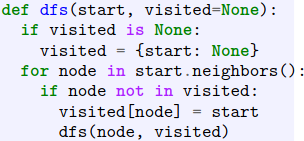
\includegraphics[scale=0.25]{dfs.png}\\
discovery edges: the edges that we take to discover a new node\\
non-tree edges: other edges\\
back edges: the edges to an ancestor in the DFS tree\\
forward edges: the edges to a descendant node in the DFS tree\\
cross edges: the edges to a non-ancestor/non-descendant node\\
properties: discovery edges form a spanning tree of the connected component; if a node v is connected to the start node, there is a path from the start node to v in the DFS tree; visits each node and check each edge once (twice for undirected graphs); complexity is O(n+m) for n nodes and m edges
}\\
\scriptsize{BFS}\\ {\tiny explore all options in parallel, divides the nodes into level (starting node at level 0...)\\
typically implemented with a queue\\
if replace the queue with a stack, it is an iterative version of DFS\\
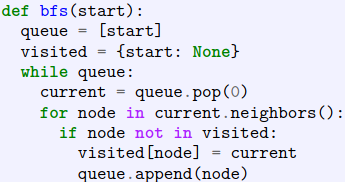
\includegraphics[scale=0.25]{bfs.png}\\
shortest path: if a node v is reachable from the start node, BFS finds the shortest path from the start node to v\\
complexity: O(n+m)
}\\
\scriptsize{find path}\\ {\tiny traverse the graph from the source code, record the discovery edges\\
start from the target node, trace the path back to the source\\
with BFS, we get the shortest path\\
running time is the length of the path O(n)\\
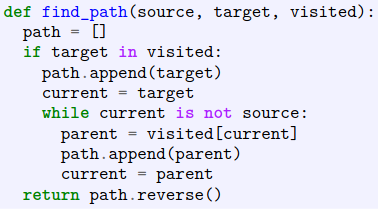
\includegraphics[scale=0.25]{find-path.png}
}\\
\scriptsize{test connectivity, find connected components, find cycle}\\
{\tiny connected: yes if the "visited" nodes have the same length as the graph nodes\\
find the connected components: run traversal multiple times until all nodes are visited\\
cyclic: yes if there is a back edge during graph traversal
}
\subsection*{Directed graphs}
\scriptsize{terminology}\\
{\tiny for any pair of nodes u and v, a directed graph is\\
strongly connected: if there is a directed path between u to v and v to u\\
semi-connected: if there is a directed path between u to v or v to u\\
weakly connected: if the undirected graph obtained by replacing all edges with undirected edges is a connected graph
}\\
\scriptsize{check strong connectivity}\\
{\tiny naive attempt: traverse the graph independently from each node (strongly connected if all traversals visit all nodes)\\
time complexity O(n(n+m))\\
better:\\ 
1. traverse the graph from an arbitrary node\\
2. reverse all edges, traverse again\\
3. intuition: if there a reverse path from D to A, then D is reachable from A\\
time complexity: O(n+m)
}\\
\scriptsize{transitive closure} {\tiny another graph where:\\
-the set of nodes are the same as the original graph\\
-there is an edge between two nodes u and v if v is reachable from u\\
for undirected graph, can be computed by computing the connected components\\
a straightforward algorithm:\\
1. run n graph traversals from each node in the graph\\
2. add an edge between the start node to any node discovered by the traversal\\
time complexity O(n(n+m))\\
(note: in a dense graph m is O(n**2))\\
Floyd-Warshall algorithm: efficient if graph is implemented with an adjacency matrix and is not sparse\\
1. setting transitive closure to the original graph\\
2. for k=1...n, add a directed edge (vi,vj) to transitive closure if it already contains both (vi,vk) and (vk,vj)\\
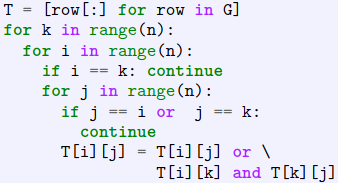
\includegraphics[scale=0.25]{floyd-warshall.png}\\
time complexity O(n**3)\\
a version of this is used for finding shortest paths in weighted graphs
}\\
\scriptsize{Directed acyclic graphs(DAGs)} {\tiny directed graphs without cycles\\
applications: course dependence, class inheritance, scheduling constrains over tasks in a project, dependency parser output\\
topological order: a sequence of nodes such that for every directed edge (u,v) u is listed before v; there may be multiple topological orderings, e.g. any acceptable order that the courses can be taken\\
topological sort:\\
1. keep record of number of incoming edges\\
2. a node is ready to be placed in the sorted list if there are no unprocessed incoming edges\\
time complexity O(n+m)\\
if topological ordering does not contain all the edges, the graph includes a cycle\\
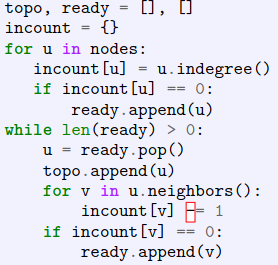
\includegraphics[scale=0.25]{topo-sort.png}
}
\subsection*{Shortest Paths}
\scriptsize{weighted graph}
{\tiny weights can be any numeric value, but some algorithms require non-negative weights or Euclidean weights (weights that are proper distance metrics)\\
weights often indicate distance or cost, but can also represent positive relations (e.g. affinity between nodes)\\
weight of a path: the sum of weights of the edges on the path
}\\
\scriptsize{shorted paths}\\
{\tiny applications: navigation, routing in computer networks, optimal construction of electronic circuits, robotics, transportation, finance...\\
shortest path on unweighted graphs: a BFS search tree\\
shortest path on unweighted graphs: different versions of the problem, restrictions on weights
}\\
\scriptsize{Dijkstra's algorithm} {\tiny a weighted version of BFS, finds shorted path from a single source node to all connected nodes\\
weights have to be non-negative\\
a greedy algorithm, grows a 'cloud' of nodes for which we know the shortest paths from the source node\\
new nodes are included in the cloud in order of their shortest paths from the source node\\
1. maintain a list D of minimum known distances to each node\\
2. at each step:\\
-take closest node out of Q\\
-update the distances of all nodes\\
3. can be more efficient if Q is implemented using a priority queue\\
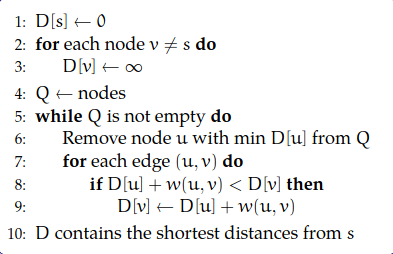
\includegraphics[scale=0.2]{Dijkstra_algo.png}
\\
complexity: in general $O(t_{find-min}n+t_{update-key}m)$\\
with list-based implementation of Q: O(m+n**2)=O(n**2)\\
with a priority queue: O((m+n)logn)\\
similar to traversal algorithms, does not give the shortest-path tree, but can be extracted from distances D, running time O(n**2) or O(n+m)\\
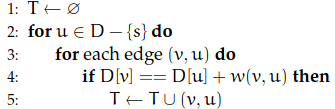
\includegraphics[scale=0.2]{path_tree.png}
\\
}
\scriptsize{Shortest paths on DAGs}
{\tiny directed acyclic graphs\\
similar to Dijkstra's, but simpler and faster\\ 
only difference is to follow a topological order\\
will also work with negative edge weights
}\\
\scriptsize{Bellman-Ford algorithm}
{\tiny single-source shortest path problem for directed graph\\
include cycles, negative weights, exclude negative cycles\\ 
1. similar to earlier algorithms, initialize D[s]=0, D[v]=infinity\\
2. make n passes over the edges:\\
-update distances for each edge (relax edges)\\
-stop if there were no changes at the end of a pass
}
\subsection*{Minimum Spanning Tree}
\scriptsize{spanning tree}\\
{\tiny - spanning graph: includes all nodes\\
tree - acyclic, connected
}\\
\scriptsize{minimum spanning tree}\\
{\tiny applications: network design, cluster analysis, traveling salesman problem, object/network recognition in images, avoidig cycles in broadcasting, dithering in images audio video, error correction codes, dna sequencing
}\\
\scriptsize{'cut property'}\\ {\tiny a cut of a graph is a partition that divides its nodes into two disjoint (non-empty) sets\\
given any cut, the edge with the lowest weight across the cut is in the MST
}\\
\scriptsize{Prim-Jarnik algorithm} {\tiny
greedy algorithm, finding MST for weighted undirected graph\\
1. starts with a single 'start' node, grows the MST greedily\\
2. at each step:\\
-consider a cut between nodes visited and the rest of the nodes\\
-select the minimum edge across the cut\\
3. repeat the process until all nodes are visited\\
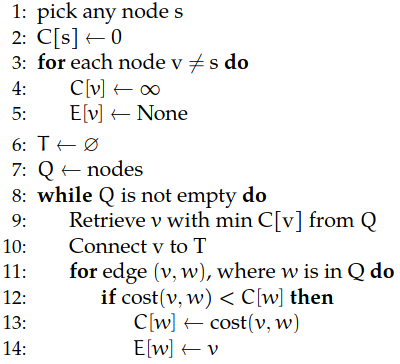
\includegraphics[scale=0.2]{prim-jarnik.png}
\\
complexity: two loops over number of nodes, O(n**2) if we need to search\\
if use a priority queue for Q, O(mlogm)\\
with a priority queue: O((m+n)logn)
}\\
\scriptsize{Kruskal's algorithm}
{\tiny finding MST on undirected graphs\\
1. start with each node in its own partition\\ 
2. at each iteration, choose the edge with the minimum weight across any two clusters, and join them\\
3. terminates when there are no clusters to join\\
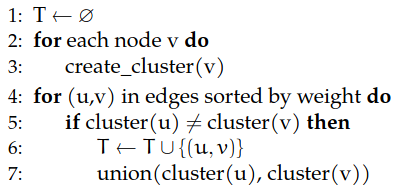
\includegraphics[scale=0.2]{kruskals_algo.png}
\\
loop over edges, but beware of the sorting requirement\\
O(mlogm) with simple data strcutures
}\\
\scriptsize{Directed trees}\\
{\tiny -rooted directed tree (arborescence): an acyclic directed graph where all nodes are reachable from the root node through a single directed path (what computational linguists simply calls a tree)\\
- anti-arborescence: a rooted directed tree where all edges are reversed\\ 
- polytree (a drected tree): a directed graph where undirected edges form a tree\\
finding an MST in a directed graph = finding a rooted directed tree
}\\
\scriptsize{Chu-Liu/Edmonds algorithm}\\
{\tiny 1. the MST for a directed graph has to start from a designated root node\\
- if selected node has any incoming edges, remove them\\ 
- common practice to introduce an artificial root node with equal-weight edges to all ndoes\\
2. for all non-root nodes, select the incoming edge with lowest weight, remove others\\
3. if the resulting graph has no cycles, it is an MST
4. if there are cycles, break them\\
- consider the cycle as a single node
- select the incoming edge that yields the lowest cost if used for breaking the cycle
5. repeat until no cycles remain\\
generally defined recursively: at each step, create a new graph with a contracted cycle call the procedure with the new graph\\
at most n recursions: the cycle has to include more nodes at every step\\
at each call, m steps for finding minimum incoming edge (also finding a cycle with O(n), but m>=n)\\
the vanilla algorithm runs in O(mn), there are improved versions\\
in CL dependency parsing:\\
1. begin with fully connected weighted graph, except the root node has no incoming edges\\
2. weights are estimated from a treebank, typically determined by a machine learning method trained on a treebank\\
3. often use probabilities, i.e. maximize the weight of the tree\\
4. one of the most common (and successful) approaches to dependency parsing
}